\documentclass[12pt,a4paper,spanish]{article}

\usepackage[utf8]{inputenc}
\pagestyle{headings}
\usepackage{babel}
\usepackage{xcolor}
\usepackage{amsmath}
\usepackage{amsfonts}
\usepackage{amssymb}
\usepackage[pdftex]{graphicx}
\usepackage[unicode=true] {hyperref}
\usepackage[toc, page, header]{appendix}

\makeatletter

%%%%%%%%%%%%%%%%%%%%%%%%%%%%%% LyX specific LaTeX commands.
\pdfpageheight\paperheight
\pdfpagewidth\paperwidth

\title{\textbf{RNAemo}\\ \vspace{0.45cm} Especificación de Diseño de Software} 
\author{Franco Gaspar Riberi}

\begin{document}
\maketitle\pagebreak{}\tableofcontents{}\pagebreak{}

\newpage

\section{Introducción}
\subsection{Propósito}

El propósito de este documento es la especificación de
diseño de software correspondiente a la primera versión del producto 
\emph{\textbf{RNAemo}}.

La confección de este documento se contextualiza dentro del desarrollo de la tesis
de grado de la carrera Licenciatura en Ciencias de la Computación de la UNRC,
\emph{\textbf{RNAemo}}, a cargo de Franco Gaspar Riberi, con la dirección
de la Lic. Laura Tardivo (UNRC) y las colaboraciones de Daniel
Gutson, y el Dr. Roberto Daniel Rabinovich
(\textbf{FuDePAN}).

El documento esta dirigido a las personas involucradas en el desarrollo de la
tesis como así también a todos los colaboradores de \textbf{FuDePAN} que eventualmente
podrían participar en las etapas de desarrollo y mantenimiento del software.

\subsection{Descripci\'on general del documento}
En la sección ~\ref{consideraciones} se mencionan los objetivos, la
metodología adoptada y las dependencias del diseño.

En la sección ~\ref{highLevel} se exhibe la arquitectura general del
sistema con sus principales componentes e interacciones.

En la sección ~\ref{middleLevel} se presenta el diseño de medio nivel del sistema,
sus interfaces y paquetes principales.
				    
En la sección~\ref{fud} se observa la paralelización del sistema empleado \emph{FuD}. 

\section{Consideraciones de diseño}
\label{consideraciones}

\subsection{Objetivos}
Se pretende lograr un diseño del sistema que cumpla con los principios
fundamentales del diseño orientado a objetos, comúnmente conocidos por el
acrónimo \textbf{``SOLID''} \cite{martin}.

En particular, se pretenden respetar los principios \textbf{SRP}
(\textit{Single Responsability Principle}), \textbf{OCP} (\textit{Open-Closed
Principle}) y \textbf{DIP} (\textit{Dependency Inversion Principle})
debido a su importancia para obtener un sistema f\'acilmente extensible
y configurable con el fin de satisfacer las necesidades de los usuarios.
  
\subsection{Metodología}
La metodología empleada para realizar el análisis y descripción del
diseño se denomina \emph{``Diseño dirigido por responsabilidades''}\cite{rebecca}. 

Esta técnica se enfoca en \textit{qué} acciones
(responsabilidades) deben ser cubiertas por el sistema 
y que objetos serán los responsables de llevarlas a cabo.
\textit{Cómo} se realizara cada acción, queda en un segunda plano.

\subsection{Herramientas y convenciones}
Se utiliza UML\cite{uml} como lenguaje de modelado, ArgoUML\cite{argoUML}, \\
\textcolor{blue}{http://www.websequencediagrams.com}
como herramientas para la confección de diagramas, y Dia\cite{dia} para la edición
de diagramas de propósito general. Además se adopta la convención de nombrar a
 las interfaces anteponiendo una letra \textit{``I''} al nombre de la clase concreta
que la implementa. \\
Por ejemplo, interface: \textit{``IPersona''} $\to$
clase concreta: \textit{``Persona''}.

\section{Diseño de alto nivel}
\label{highLevel}
La arquitectura del sistema y la interacción entre los diversos componentes que la conforman se exhiben en la figura~\ref{arquitecture}. En las subseccones siguientes se describe brevemente cada uno de ellos.

\begin{figure}[!hbtp]
	\begin{center}
		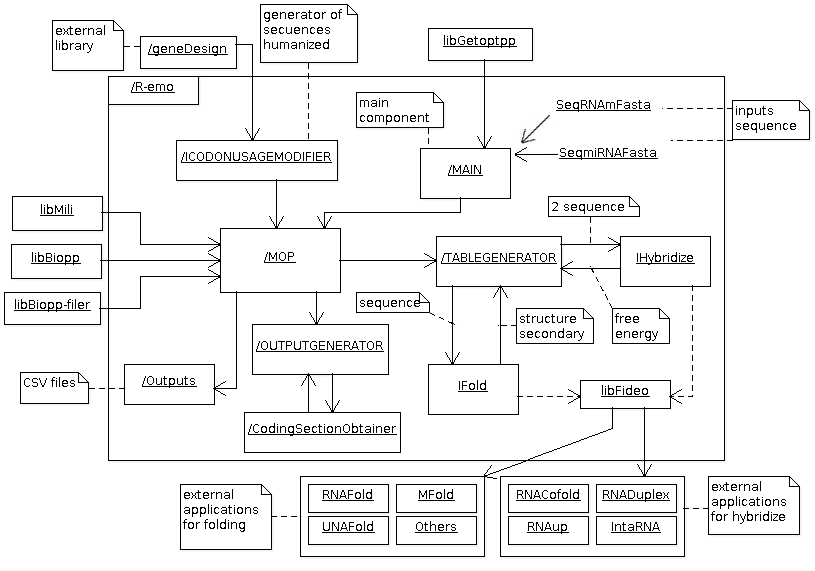
\includegraphics[width=20cm, height=12cm, angle=90]{image/architecture.png}
		\caption{UML - Arquitectura del Sistema}
		\label{arquitecture}
	\end{center}
\end{figure}

\subsection{Componetes del sistema}
   \begin{itemize}
      \item \textbf{Main:} corresponde al módulo principal en términos de ejecución del sistema.

      \item \textbf{MasterOfPuppets (MOP):}  comprende la inicialización e invocación de los demás
      componentes. Coordina y gestiona la mayoría de las interacciones entre módulos.
    
      \item \textbf{ICodonUsageModifier:} interface que permite la humanización de secuencias.  

      \item \textbf{GeneDesign:} representa el componente encargado de generar secuencias humanizadas. Dada
      una secuencia original, genera la secuencia humanizada correspondiente. Dicho módulo es externo a este
      desarrollo, y para ello se emplea el software \emph{GeneDesign}.

      \item \textbf{OutputsGenerator:} comprende la generación de archivos. Se crean tanto archivos como 
      RNA$_m$ se analizen.

      \item \textbf{CodingSectionObtainer:} componente que permite obtener la sección codificante específica. 
		
      \item \textbf{TableGenerator:} este componente es el encargado de rellenar las tablas. Para ello,
      realiza el matching por complemento y el cálculo de score entre secuencias de RNA$_m$ y small-RNA$_s$. 

      \item \textbf{IFold:} representa la interface encargada del folding de secuencias.

      \item \textbf{IHybridize:} corresponde a la interface encargada de la hibridización de secuencias.
   \end{itemize}

\subsection{Librerias externas}
\begin{itemize}
    \item \textbf{Mili:} corresponde a una colección de funciones de C++, para resolver detalles de
     implementación.

    \item \textbf{fideo:} corresponde a una librería parcialmente ya implementada. Provee al sistema la
     funcionalidad de \emph{``folding''} e hibridación. 

    \item \textbf{Biopp:} biblioteca C++ para Biología Molecular. Permite la manipulación de secuencias de
    ácidos nucleicos.  

    \item \textbf{Biopp-filer:} para la lectura de secuencias en formato FASTA.    

    \item \textbf{getoptpp} para facilitar el manejo de entrada estándar.
\end{itemize}

\subsection{Interacción entre los componentes}
En la figura~\ref{mensajes} se presenta la interacción entre componentes a través de un diagrama de secuencias. Se empleó este tipo de diagrama ya que permite capturar en forma óptima la secuencia temporal de las interacciones entre los componente.

\begin{figure}
  \centering
  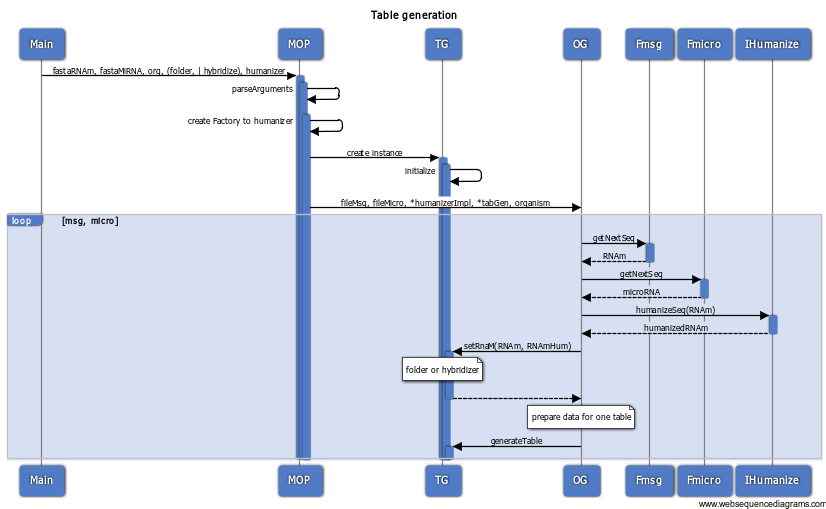
\includegraphics[scale=0.6, angle=90]{image/seqDiagrams.png}  
  \caption{UML - Diagrama de secuencia}
  \label{mensajes}
\end{figure}

\section{Diseño de medio nivel}
\label{middleLevel}
\subsection{Estructura de paquetes}
La figura~\ref{package} muestra los diferentes paquetes que conforman el sistema.
\begin{figure}
  \centering
  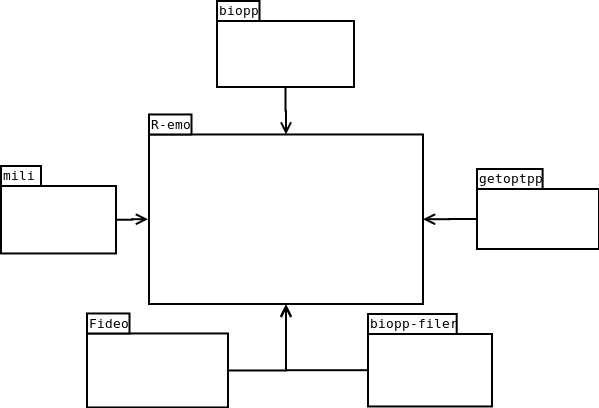
\includegraphics[scale=0.65]{image/packageDiagramHighGranularity.png}  
  \caption{UML - Paquetes}
  \label{package}
\end{figure}

\vskip 5cm

\subsection{Diagrama de clases}
\begin{figure}
  \centering
  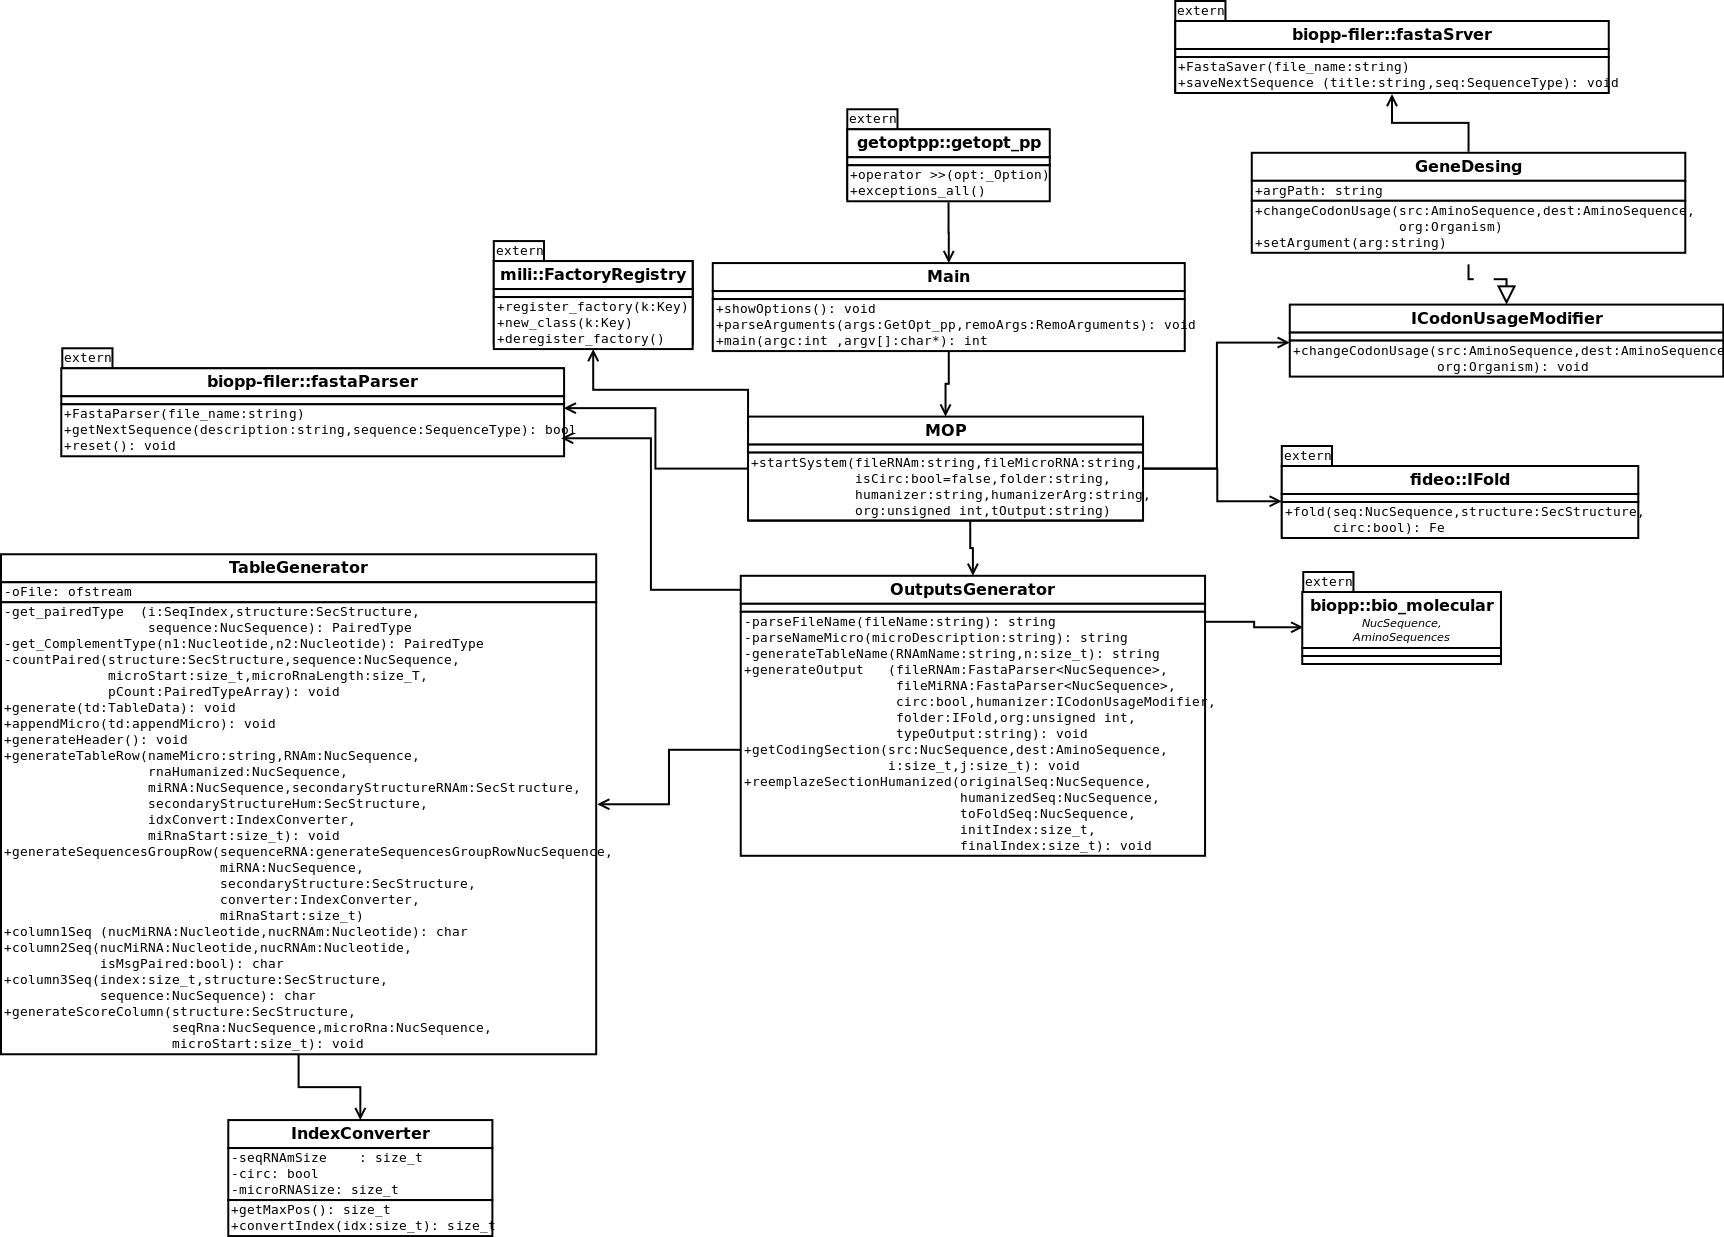
\includegraphics[scale=0.35, angle=90]{image/ClassDiagram.png}  
  \caption{UML - Diagrama de clases}
  \label{clases}
\end{figure}

\subsection{Clases}
\subsubsection{Interfaces}
\begin{itemize}
    \item \textbf{fideo:}
        \begin{itemize}
            \item \emph{IFold:} describe de manera transparente el servicio de folding.
            \item \emph{IHybridize:} describe de manera transparente el servicio de hibridación.
        \end{itemize}
    \item \textbf{ICodonUsageModifier:} describe de manera transparente el servicio de humanización de
                                        secuencias.
\end{itemize}

\subsubsection{Clases concretas}
\begin{itemize}
    \item \textbf{fideo:}
        \begin{itemize}
            \item \emph{RNAFold y UNAFold:} backends específicos para folding.
            \item \emph{RNAup, RNAcofold, RNAduplex e IntaRNA:} backends específicos para hibridar.
        \end{itemize}
    \item \textbf{GeneDesign:} software específico (geneDesign) para humanizar.
\end{itemize}

\subsection{Interfaces - Responsabilidades - Colaboradores}
En esta sección se presentan las principales interfaces que intervienen en el sistema, sus respectivas responsabilidades y colaboradores. 

\begin{itemize}
    \item \textbf{Module:} MOP \\
    \textbf{Target:} Gestionar la iteración de módulos. \\
    \textbf{Responsibilities:} Interconectar partes del sistema. \\
    \textbf{Services:} 
        \begin{itemize}
            \item Creación de objetos necesarios.
            \item Invocación a humanización.
            \item Invocación a folding secuencia original.
            \item Invocación a folding secuencia humanizada.
            \item Invocación al generador de archivos.
        \end{itemize}
    \textbf{Collaborations:}	GeneDesign, OutputsGenerator , TableGenerator. \\

    \item \textbf{Module:} Main. \\
    \textbf{Target:} Lanzar la aplicación. \\
    \textbf{Responsibilities:} Lanzador de aplicación. \\
    \textbf{Services:}
        \begin{itemize}
            \item Mostrar opciones de uso.
            \item Parsear los argumentos de entrada.
            \item Capturar las excepciones ocurridas durante la ejecución.
        \end{itemize} 
    \textbf{Collaborations:} MOP. \\

    \item \textbf{Module:} GeneDesign. \\
    \textbf{Target:}  Humanizar secuencias. \\
    \textbf{Responsibilities:} Humanizar una secuencia de RNA. \\
    \textbf{Services:}
        \begin{itemize}
            \item Setear el path del software humanizador.
            \item Humanizar una secuencia.
        \end{itemize} 
    \textbf{Collaborations:}	- \\

    \item \textbf{Module:} OutputsGenerator. \\
    \textbf{Target:} Generador de archivos. \\
    \textbf{Responsibilities:} Construir un archivo de salida. \\
    \textbf{Services:}
        \begin{itemize}
            \item Generar el nombre de cada archivo.
            \item Parsear la descripcion de cada Fasta.
            \item Generar un archivo por cada RNAm-miRNA.
        \end{itemize} 
    \textbf{Collaborations:} TableGenerator. \\

    \item \textbf{Module:} TableGenerator. \\
    \textbf{Target:} Construir tablas. \\
    \textbf{Responsibilities:} Rellenar una tabla. \\
    \textbf{Services:}
        \begin{itemize}
            \item Generar el encabezado de una tabla.
            \item Generar fila de scores.
            \item Generar fila de matching (complemento, enmascarados).
            \item Escribir una linea de la tabla.
            \item Calcular cada columna de la tabla.
            \item Contabilización de nucleótidos apareados.
            \item Escritura en un archivo.
        \end{itemize} 
    \textbf{Collaborations:} - \\
\end{itemize}

\section{Fud-agnostic}
\label{fud}

\par El componente principal \textsf{MasterOfPuppets} será el encargado de la generación de las tablas. Para ello, se implementará un método \textsf{generateTable}, el cual tomará como parámetro el RNA mensajero, el RNA humanizado y un $_m$$_i$RNA. El componente principal realizará una doble iteración anidad entre RNA$_m$ y $_m$$_i$RNA. Es decir, por cada RNA$_m$ se recorrerá cada secuencia de $_m$$_i$RNA invocando al método ya mencionado.

\par Esto permitirá un paralelización trivial empleando \emph{FuD}.

\begin{center}
\textsf{generateTable (const Sequence\& rna\_original, const Sequence\& rna\_humanized, const Sequence\& mi\_rna)}
\end{center}


\begin{thebibliography}{99}
\small  \bibitem{martin} {\em{“Design Principles and Design Patterns.”}} 
		\textsc{Robert C. Martin}, 2000. \textcolor{blue}{http://www.objectmentor.com}
  
\small  \bibitem{rebecca} {\em{“Object Design: Roles, Responsibilities.”}} 
		\textsc{Rebecca Wirfs-Brock and Alan McKean and Collaborations}, Addison-Wesley, 2003.  

\small  \bibitem{uml} {\em{“Unified Modeling Language.”}} \textcolor{blue}{http://www.uml.org/}

\small  \bibitem{argoUML} {\em{“ArgoUML.”}} \textcolor{blue}{http://argouml.tigris.org/}

\small \bibitem{dia} {\em{“Dia.”}} \textcolor{blue}{http://live.gnome.org/Dia}
\end{thebibliography}

\end{document}
